\documentclass{endm}
\usepackage{endmmacro}
\usepackage{graphicx}
\usepackage{float}
\usepackage[utf8]{inputenc}
\usepackage[spanish,activeacute]{babel}
\usepackage{setspace}  
\setlength{\textwidth}{150mm}

% The following is enclosed to allow easy detection of differences in
% ascii coding.
% Upper-case    A B C D E F G H I J K L M N O P Q R S T U V W X Y Z
% Lower-case    a b c d e f g h i j k l m n o p q r s t u v w x y z
% Digits        0 1 2 3 4 5 6 7 8 9
% Exclamation   !           Double quote "          Hash (number) #
% Dollar        $           Percent      %          Ampersand     &
% Acute accent  '           Left paren   (          Right paren   )
% Asterisk      *           Plus         +          Comma         ,
% Minus         -           Point        .          Solidus       /
% Colon         :           Semicolon    ;          Less than     <
% Equals        =           Greater than >          Question mark ?
% At            @           Left bracket [          Backslash     \
% Right bracket ]           Circumflex   ^          Underscore    _
% Grave accent  `           Left brace   {          Vertical bar  |
% Right brace   }           Tilde        ~

\newcommand{\Nat}{{\mathbb N}}
\newcommand{\Real}{{\mathbb R}}
\begin{document}
% DO NOT REMOVE: Creates space for Elsevier logo, ScienceDirect logo
% and ENDM logo
\begin{verbatim}\end{verbatim}\vspace{.5cm}
\begin{frontmatter}
\title{Las Reglas del Congreso}
\author{Diego Santos\thanksref{sdemail}}
\author{Axel Savizky  \thanksref{raemail}}
\address{Reglas de Asociación y Simulación de Patrones - Departamento de Computación - Universidad de Buenos Aires - Bs.As., Argentina}
\thanks[raemail]{Email:
  \href{mailto:axel.savizky@gmail.com} {\texttt{\normalshape
   axel.savizky@gmail.com}}}
\thanks[sdemail]{Email:
  \href{mailto:diego.h.santos@gmail.com} {\texttt{\normalshape
   diego.h.santos@gmail.com}}}
\begin{abstract}
Todos los años durante el período de marzo a diciembre 257 diputados se reunen para determinar que nuevas leyes regirán sobre el pueblo argentino. En el presente trabajo se analizó un conjunto de votaciones de la Cámara de Diputados de la Nación con el fin de identificar las reglas que se esconden en las sanciones de leyes.
\end{abstract}
\begin{keyword}
Diputados, Transacciones, Monotonía, Leyes, Ausencias.
\end{keyword}
\end{frontmatter}
\section{Presentación}\label{intro}
El objetivo del trabajo es determinar reglas en las votaciones de ley de la Cámara de Diputados del Congreso de la Nación Argentina a partir de los resultados de las votaciones de cada ley correspondientes al período de marzo a septiembre de 2018.\\

Durante este período se trataron 72 leyes, involucrando a cada una 257 diputados de 32 partidos poltíticos agrupados en 17 interbloques.\\

La datos para la confección del reporte se obtuvieron de la página web de la Cámara de Diputados. \footnote{https://www.diputados.gov.ar/}

\subsection{Set de Datos}

El set de datos utilizado consta de 72 archivos csv donde en cada uno de ellos se muestra por fila: \\

Diputado $|$ Partido $|$ Provincia $|$ ¿Cómo voto?\\

Es decir que cada archivo tiene 257 filas donde en cada una se presenta un diputado, el partido al que pertenece, la provincia a la que representa y cual fue su voto.\\

El campo ¿Cómo voto? tiene 5 estados posibles:\\

\begin{itemize}
\item Presidente: Si ejerció como presidente de la sesión.
\item Afirmativo: Si su voto a favor de la sanción de la ley.
\item Negativo: Si su voto fue en contra de la sanción de la ley.
\item Abstención: Si se excuso de votar.
\item Ausente: Si no estuvo presente en el recinto.
\end{itemize}

\subsection{Transacción}

Los datos en el formato que se obtuvieron no resultan útiles para establecer reglas más allá de las evidentes, por lo que fue necesario reagrupar los datos en otro tipo de transacción. \\

De un análisis de los datos en crudo se descubrió que en casi la totalidad de los casos la votación de los diputados es en bloque. Es decir, siguen una disciplina partidaria donde todos los pertenecientes al mismo partido votan igual, sin importar la provincia a la que pertenezcan. Además dicha disciplina suele aplicarse también para los interbloques. \\

Entonces el voto de un diputado esta condicionado a la decisión del partido y no esta condicionado por la provincia a la que representa. Entonces para el armado de la transacción se consideró que no es necesario contar con el nombre del diputado, sino por como voto su partido esa ley. \\

Además como cada provincia esta representada por un subconjunto de diputados, proporcional a la población de dicha provincia, que pertenecen a un subconjunto de los partidos, se determino que una forma conveniente de representar la decisión de la provincia es tomando el valor de la mayoría de los votos de los diputados que la representan. \\

En base a esto se decidió construir la transacción con el siguiente formato: \\

Ley $|$ Estado $|$ Partido1 $|$...$|$ Partido32 $|$ Provincia1 $|$ ... $|$ Provincia22 \\

Donde el valor de cada campo columna puede tomar los siguientes valores: \\

Para \textbf{Ley} \\

El nombre de archivo csv que corresponde al dataset de un tratamiento de ley. \\

Para \textbf{Estado} \\

\begin{itemize}
\item $LEY APROBADA$: Si la ley fue aprobada.
\item $LEY RECHAZADA$: Si la ley no fue aprobada. \\
\end{itemize}

 Para \textbf{Partido X} \\

\begin{itemize}
\item $PARTIDO [AFIRMATIVO]$
\item $PARTIDO [NEGATIVO]$
\item $PARTIDO [ABSTENCION]$
\item $PARTIDO [AUSENTE]$ 
\item $PARTIDO [EMPATE]$ \\
\end{itemize}

Donde el valor se define siguiendo el criterio de las mayorías. Para la ley que presenta la transacción se contabilizan los votos de todos los diputados del partido
y se asigna el resultado de la mayoria. EMPATE se utiliza si no hay un criterio mayoritario. \\

Por ejemplo: \\

Partido1 que tiene 5 diputados representantes, 4 votan afirmativo y 1 ausente, al haber mas votos positivos el resultado es PARTIDO1 [AFIRMATIVO] \\

Partido2 que tiene 2 diputados representantes, 1 vota afirmativo y otro 1 ausente. El resultado es PARTIDO1[EMPATE] \\

Para \textbf{Provincia X} \\

\begin{itemize}
\item $PROVINCIA [AFIRMATIVO]$
\item $PROVINCIA [NEGATIVO]$
\item $PROVINCIA [ABSTENCION]$
\item $PROVINCIA [AUSENTE]$ 
\item $PROVINCIA [EMPATE]$ \\
\end{itemize}

Donde el valor se define siguiendo el criterio de las mayorías. Para la ley que presenta la transacción se contabilizan los votos de todos los diputados que pertenecen a esa provincia, sin considerar el partido y se asigna el resultado de la mayoria. EMPATE se utiliza si no hay un criterio mayoritario. \\

Por ejemplo: \\

Una provincia que tiene 2 partidos que la representan en el recinto. El Partido1 tiene 5 diputados, 4 votan afirmativo y 1 ausente. El Partido2 tiene 3 diputados que votan de forma negativa. El resultado es PARTIDO1 [AFIRMATIVO]. \\

Esta representación de transacción permite clusterizar los datos individuales de cada diputado evitando la redundancia de datos permitiendo obtener reglas generalizadas sobre los partidos y los interbloques a los que pertenecen. \\

El motivo por el que las ausencias son consideradas en el armado de la transacción es que la presencia o no de un bloque en ciertos casos puede ser parte del armado de una estrategia legislativa, especialmente en los partidos que no son un monobloque.

\newpage 

\section{Reglas}\label{desarrollo}

Para encontrar las reglas que determinan el comportamiento del set de transacciones se utilizó la implementación del algoritmo $Apriori$ del paquete aRules del lenguaje de programación $R$.\\

El objetivo es a partir de las reglas encontradas, describir el comportamiento que lleva a que una ley sea aprobada o rechazada, para facilitar la descripción se analizan por separado las reglas por separado para luego sobre el fin del trabajo, para luego sobre el fin del trabajo establecer las reglas sobre la sanción o rechazo de la ley.\\

De las reglas obtenidas se presenta un análisis de las consideradas más relevantes para describir la dinámica de la Cámara Baja. \\

En la sección de $Diputados$ se describen las reglas que siguen los diputados en relación al partido que pertenecen.\\

En la sección de $Partidos$ se describen las reglas que relacionan a un partido con otro. Es decir que partidos votan frecuentemente de la misma forma o de forma opuesta.\\

En la sección de $Interbloques$ se describen las reglas que relacionan a los partidos del mismo interbloque y luego las del interbloque en conjunto contra los demás partidos.\\

En la sección de $Provincias$ se describen las reglas que relacionan a las provincias entre sí.\\

En la sección de \textit{Partidos y Provincias} se describen las reglas que relacionan a los partidos con las provincias.\\

En la sección de \textit{Sanciones de Ley} se describen las reglas son las que llevan a la aprobación o rechazo de una ley.\\

Para una mejor visualización e interpretación de las reglas es conveniente intercalar la lectura de esta sección con la infografía de leyes detallada en el archivo \textbf{$infografia leyes.html$} la cual permite explorar la totalidad de las reglas de las secciones antes mencionadas. Dentro de la carpeta \textbf{$reglas XML$} se encuentran en formato xml un conjunto de archivos que contienen todas las reglas obtenidas para cada sección.\\

Para una mayor simplicidad de análisis en cada una de las secciones de estudio se limito el dataset a los items a estudiar en cada sección. El objetivo fue procesar menos datos para obtener resultados enfocados al estudio de la sección, además de una mayor simplicidad en el script que genera las reglas.\\

Como parametros del algoritmo apriori se asigna confidence = 0.80, pues interesa encontrar patrones muy frecuentes. El valor del soporte será estudiado para cada sección dependiendo del dataset. \\

Los dataset puede encontrarse en la seccion /datos. \\

\subsection{Diputados}

Del análisis exploratorio de los datos en crudo se pudo observar y determinar que un diputado perteneciente a un partido cualquiera vota de la misma forma que el resto de sus compañeros de partido. Este comportamiento se repite en 71 de las 72 sesiones analizadas.\\

Sin importar la provincia a la que represente, un diputado vota alineado al partido al que pertenece.\\


\subsection{Partidos}

En esta sección se presentan las reglas que involucran a los partidos. La intención es establecer reglas que permitan inferir que partidos votan alineados y quienes lo hacen de forma opuesta. \\

El dataset utilizado es transaccionespartidos.csv. Se analiza la distribución de los datos para encontrar un valor para el soporte del algoritmo apriori. \\

\begin{center}
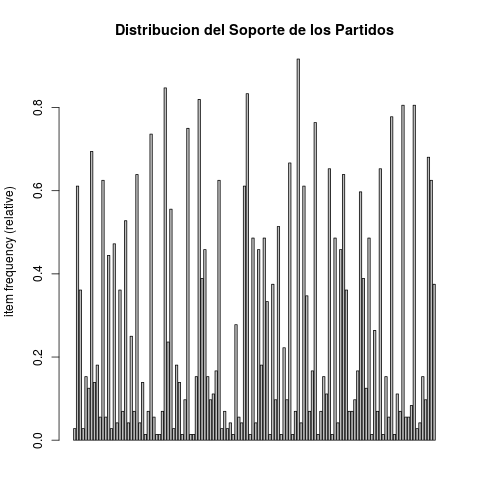
\includegraphics[scale=0.4]{graficos/soportesPartidos.png} \\
\end{center}

\textit{Entre dos Partidos} \\

Debido a la gran cantidad de datos para esta sección el parámetro de confianza para el algoritmo de apriori será de 0.90 y el soporte de 0.60. \\

Se obtuvieron 42 reglas que pueden encontrarse en el archivo reglasPartidos.xml.  \\

Se considerán destacables las siguientes reglas respecto al partido oficialista: \\

{Coalicion Civica[NEGATIVO]} $\Longrightarrow$ {PRO[NEGATIVO]} \\

Con un soporte de 0.61, confianza 1 y lift 1.5.\\

{Partido por la Justicia Social[NEGATIVO]} $\Longrightarrow$ {PRO[NEGATIVO]} \\

Con un soporte de 0.61, confianza 1 y lift 1.5.\\

{Union Civica Radical[NEGATIVO]}  $\Longrightarrow$ {PRO[NEGATIVO]}\\

Con un soporte de 0.62, confianza 1 y lift 1.5.\\

Al darse el voto negativo de estos partidos es esperable que también el PRO vote de la misma forma. Cabe destacar que estos partidos se encuentran dentro del mismo interbloque, por lo que es esperable que sus votos estén en síntonia. \\

{PRO[NEGATIVO]}  $\Longrightarrow$ {Frente\ para\ la\ Victoria - PJ[POSITIVO]} \\

Con un soporte de 0.61, confianza de  0.95 y lift 1.16. Es esperado que el voto del Frente para la Victoria - PJ sea opuesto al del PRO, confirmando la coyuntura política del país. \\ 

También son destacables las reglas sobre los partidos que pueden englobarse dentro del denominado $Peronismo$ \\

{Justicialista por Tucuman[POSITIVO]} $\Longrightarrow$ {Justicialista[POSITIVO]} \\

Con un soporte de  0.61, confianza 1 y lift 1.2\\

{Peronismo para la Victoria[POSITIVO]} $\Longrightarrow$ {Frente\ para\ la\ Victoria - PJ[POSITIVO]}  \\

Con un soporte de 0.61, confianza 0.93y lift 1.14\\

{Unidad Justicialista[POSITIVO]}  $\Longrightarrow$ {Justicialista[POSITIVO]} \\

Con un soporte de 0.62, confianza 0.91 y lift 1.10\\

{FPV - PJ[POSITIVO]} $\Longrightarrow$ {Federal\ Unidos\ por\ una\ Nueva\ Argentina[POSITIVO]}\\

Con un soporte de 0.76, confianza 0.93 y lift 1.10\\

Hay una gran correlación entre sus votos, si bien en estos casos la relación es 1 a 1, se espera que mas adelante se confirme la tendencia a votar similar entre las muchas vertientes del $Peronismo$.\\

Una regla que resultó inesperada teniendo en cuenta nuestros conocimientos sobre la coyuntura política argentina es: \\

{Fte. de Izquierda y de los Trabajadores[POSITIVO]} $\Longrightarrow$ {FPV - PJ[POSITIVO]}\\

Con un soporte de 0.61, confianza 0.97 y lift 1.1. A priori no era esperada tanta correlación entre el principal partido de izquierda y el FPV. \\

\textit{Entre grupo de Partidos} \\

Del grafico de distribución de los items se considero adecuado para este caso utilizar un valor de soporte de 0.65 y el valor de confianza de 0.80. \\

Se obtuvieron 92 reglas que pueden encontrarse en el archivo reglasPartidosGrupos.xml \\

\begin{center}
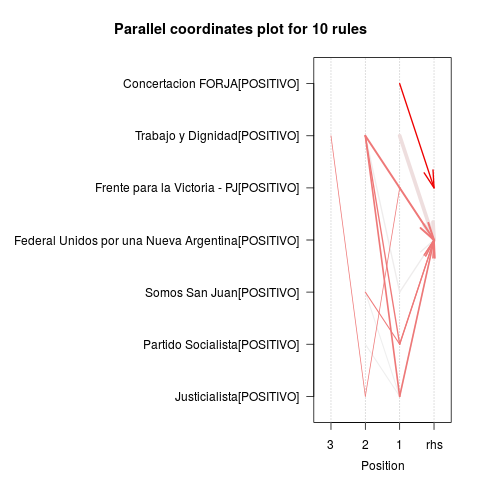
\includegraphics[scale=0.5]{graficos/paracoordPartidosGrupos.png} \\
\scriptsize{Figura: La forma en que voto un partido se representa sobre el eje y. Mientras que la intersección sobre  los números representa que se encuentra del lado izquierdo y la flecha representa cual valor se ubica en el lado derecho.} \\
\end{center} 


Es destacable un análisis sobre algunas reglas: \\

{Partido Socialista[POSITIVO], Somos San Juan[POSITIVO]} $\Longrightarrow$ \\ {Federal\ Unidos\ por\ una\ Nueva\ Argentina[POSITIVO]} \\

Con un soporte de 0.66, confianza 1 y lift 1.19. Se da que siempre que el Partido Socialista y Somos San Juan votan positivo, el Partido Unidos por una Nueva Argentina también lo hace. Lo que hace particular a esta regla es que todos los partidos pertenecen a interbloques distintos. \\


{Federal Unidos por una Nueva Argentina[POSITIVO], Frente para la Victoria - PJ[POSITIVO], Justicialista[POSITIVO], Trabajo y Dignidad[POSITIVO]}   $\Longrightarrow$ {Partido\ Intransigente\ de\ Mendoza[POSITIVO]} \\

Con un soporte de 0.65, confianza 1 y lift 1.09. El Partido Intransigente de Mendoza acompaña con el voto positivo cuando los partidos mayoritarios de la oposición votan en positivo, a pesar de no pertener a ningún interbloque. \\


Es tambien importante destacar dos nuevas reglas entre partidos que surgieron en esta etapa: \\

{Frente para la Victoria - PJ[POSITIVO]}  $\Longrightarrow$ {Justicialista[POSITIVO]} \\

Con un soporte de 0.73, confianza 0.89 y lift 1.0 \\

{FPV - PJ[POSITIVO]}  $\Longrightarrow$ {Federal\ Unidos\ por\ una\ Nueva\ Argentina[POSITIVO]} \\

Con un soporte de 0.76, confianza 0.93 y lift 1.1 \\

Esto representa que si el Frente Para la Victoria vota de forma positiva hay una gran probabilidad que de los partidos Justicialista y Federal Unidos por una Nueva Argentina también los hagan. La importancia se da porque son 3 de los 4 partidos más grandes, y no estan aglutinados en el mismo interbloque. Estos 3 partidos de forma coordinada pueden determinar la aprobación de una ley.


\subsection{Interbloques}

En esta sección se presentan las reglas que representan el comportamiento de los partidos agrupados en Interbloques.\\

Primero se presentan las reglas correspondientes a la dinámica interna del interbloque, con el fin de conocer como se comportan en bloque.El dataset utilizado para las reglas entre los miembros del interbloque contiene todos los votos de los partidos pertenecientes al interbloque. La longitud de las reglas pedidas al algoritmo son del tamaño del bloque, a fin de obtener del lado izquierdo todos los partidos menos uno, que estará del lado derecho.\\

Luego se analizan las reglas del interbloque completo con el resto de los partidos politicos. El dataset utilizado para las reglas entre el interbloque con los demás partidos contiene todos los votos de todos los partidos. En el algoritmo apriori se indico que se generen las reglas con todo el interbloque del lado izquierdo quedando del lado derecho un partido que no pertenece al interbloque. El dataset utilizado es transaccionespartidos.csv, al ser común para todos los interbloques, se presenta el grafico de distribución de los soportes de 1-itemset y luego en cada sección se determinará el adecuado.\\

\begin{center}
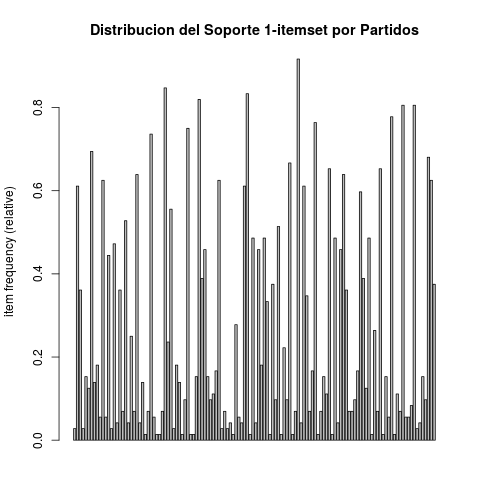
\includegraphics[scale=0.5]{graficos/soportesParaPartidos.png} \\
\scriptsize{Figura: Distribución de los items de todos los partidos.} \\
\end{center}

\newpage 

\textbf{Interbloque Cambiemos}\\

\textit{Dentro del Interbloque} \\

El dataset utilizado es transaccionescambiemos.csv. Se analiza la distribución de los datos para encontrar un valor para el soporte del algoritmo apriori. \\

\begin{center}
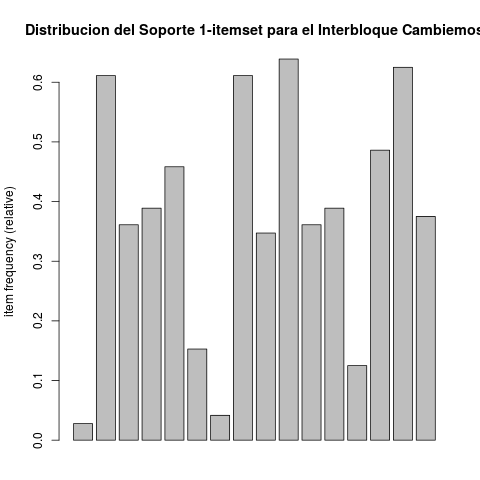
\includegraphics[scale=0.4]{graficos/soportesCambiemos.png}
\end{center}

En base a la distribución de los datos observada un valor adecuado para el soporte es 0.1.\\

Con esta configuración y luego de eliminar las reglas redundantes se obtuvieron 4 reglas. Se encuentran en el archivo reglasCambiemos.xml  \\

\begin{center}
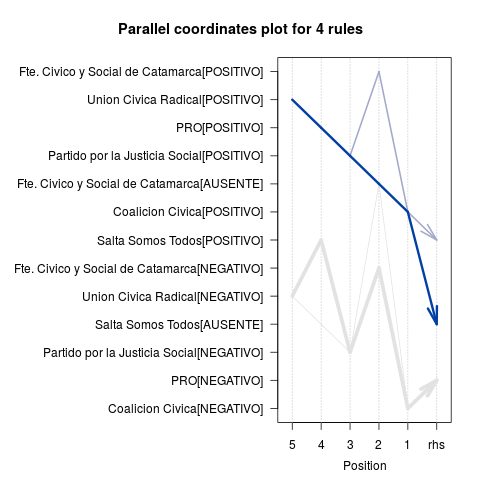
\includegraphics[scale=0.5]{graficos/paracoordInterbloquesCambiemos.png} \\
\scriptsize{Figura: La forma en que voto un partido se representa sobre el eje y. Mientras que la intersección sobre  los números representa que se encuentra del lado izquierdo y la flecha representa cual valor se ubica en el lado derecho.}
\end{center}

Se considerán destacables las reglas: \\

{Coalicion Civica[POSITIVO],
 Fte. Civico y Social de Catamarca[POSITIVO],
 Partido por la Justicia Social[POSITIVO],   
 PRO[POSITIVO], Union Civica Radical[POSITIVO]} $\Longrightarrow${Salta\ Somos\ Todos[POSITIVO]} \\

Con soporte de 0.15, confianza de 1 y lift de 2.05. Muestra  con un soporte de 0.15 que el interbloque vota en conjunto de forma positiva. \\

{Coalicion Civica[NEGATIVO],         
Fte. Civico y Social de Catamarca[NEGATIVO],
Partido por la Justicia Social[NEGATIVO],
Salta Somos Todos[POSITIVO],
Union Civica Radical[NEGATIVO]}  $\Longrightarrow$ {PRO[NEGATIVO]} \\

Con soporte de 0.26, confianza de 1 y lift de 1.56. Muestra  con un soporte de 0.15 que no vota unido de forma negativa. Sino que el partido Salta Somos Todos suele mostrarse autónomo. \\

Una curiosidad esta dada por la siguiente regla: \\

{Coalicion Civica[POSITIVO],                    
Fte. Civico y Social de Catamarca[AUSENTE], 
Partido por la Justicia Social[POSITIVO], 
PRO[POSITIVO], 
Union Civica Radical[POSITIVO]}             $\Longrightarrow$  {Salta\ Somos\ Todos[AUSENTE]} \\

Con soporte de 0.19, confianza de 1 y lift de 2.57. Muestra que los miembros de los partidos Salta Somos Todos y Fte. Civico y Social de Catamarca suelen ausentarse juntos cuando los demás miembros votan de forma positiva. \\


\textit{Interbloque contra el resto de los partidos} \\

En base a la distribución de los datos observada un valor adecuado para el soporte es 0.25. \\

Con esta configuración y luego de eliminar las reglas redundantes se obtuvieron 9 reglas. Se encuentran en el archivo reglasCambiemosRestoPartidos.xml  \\

\begin{center}
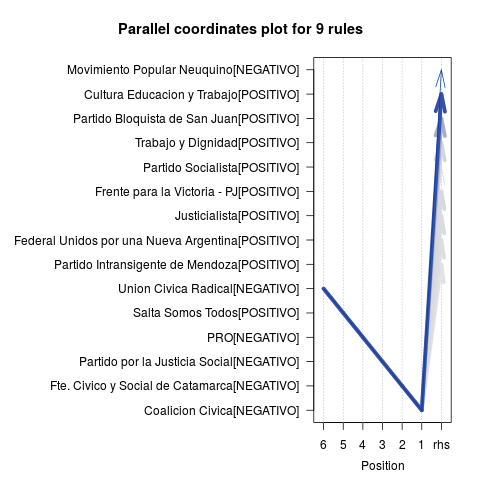
\includegraphics[scale=0.5]{graficos/paracoordCambiemosRestoPartidos.png} \\
\scriptsize{Figura: La forma en que voto un partido se representa sobre el eje y. Mientras que la intersección sobre  los números representa que se encuentra del lado izquierdo y la flecha representa cual valor se ubica en el lado derecho.}
\end{center} 

Se considerán destacables las reglas: \\

{Coalicion Civica[NEGATIVO], Fte. Civico y Social de Catamarca[NEGATIVO], Partido por la Justicia Social[NEGATIVO], PRO[NEGATIVO], Salta Somos Todos[POSITIVO], Union Civica Radical[NEGATIVO]} $\Longrightarrow$ \\ {Movimiento\ Popular\ Neuquino[NEGATIVO]} \\

Con soporte de 0.25, confianza de 0.94 y lift de 1.94. El partido Movimiento Popular Neuquino suele acompañar en el voto Negativo a la mayoria del interbloque, que vota mientras que el partido Salta Somos Todos vota de forma distinta al interbloque. \\

{Coalicion Civica[NEGATIVO],
Fte. Civico y Social de Catamarca[NEGATIVO],    
Partido por la Justicia Social[NEGATIVO],       
PRO[NEGATIVO], 
Salta Somos Todos[POSITIVO], Union Civica Radical[NEGATIVO]} $\Longrightarrow$ {FPV - PJ[POSITIVO]} \\

Con soporte de 0.26, confianza de 1 y lift de 1.22. El partido Frente para la Victoria - PJ vota de forma positiva cuando el interbloque vota de forma negativa excepto Salta Somos Todos que vota positivo.\\

De las reglas obtenidas puede deducirse que el partido Salta Somos Todos suele votar en contra del interbloque cuando este lo hace de forma negativa. Y se puede inferir que suele acompañar a la oposición a su interbloque.  \\

\newpage 

\textbf{Interbloque Frente Para la Victoria - PJ}\\

\textit{Dentro del Interbloque} \\

El dataset utilizado es transaccionesfpv.csv. Se analiza la distribución de los datos para encontrar un valor para el soporte del algoritmo apriori. \\

\begin{center}
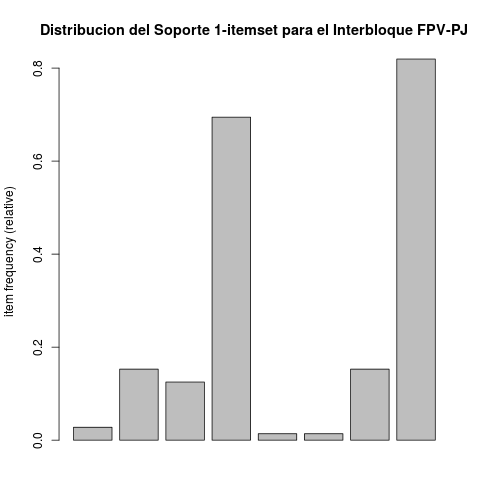
\includegraphics[scale=0.4]{graficos/soportesInterbloquesFpv.png}
\end{center}

En base a la distribución de los datos observada un valor adecuado para el soporte es 0.1.\\

Con esta configuración y luego de eliminar las reglas redundantes se obtuvieron 3 reglas. Se encuentran en el archivo reglasInterbloqueFpv.xml  \\

Las reglas que cabe descatar son \\

{Concertacion FORJA[NEGATIVO]} $\Longrightarrow$ {Frente para la Victoria - PJ[NEGATIVO]} \\

Con soporte 0.11, confianza de 0.88 y lift de 5.81 \\

{Concertacion FORJA[POSITIVO]} $\Longrightarrow$ {Frente para la Victoria - PJ[POSITIVO]} \\

Con soporte 0.68, confianza de 0.98 y lift de 1.19 \\

Los partidos del interbloque votan tanto de forma positiva como negativa de forma conjunta. \\

\textit{Interbloque contra el resto de los partidos} \\

En base a la distribución de los datos observada un valor adecuado para el soporte es 0.25. \\

Con esta configuración y luego de eliminar las reglas redundantes se obtuvieron 8 reglas. Se encuentran en el archivo reglasFpvRestoPartidos.xml  \\

\begin{center}
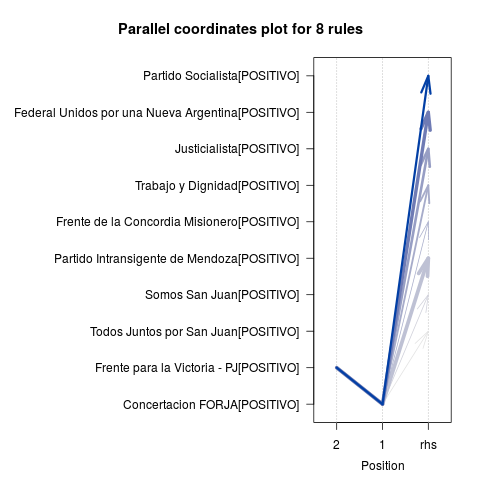
\includegraphics[scale=0.5]{graficos/paracoordFpvRestoPartidos.png} \\
\scriptsize{Figura: La forma en que voto un partido se representa sobre el eje y. Mientras que la intersección sobre  los números representa que se encuentra del lado izquierdo y la flecha representa cual valor se ubica en el lado derecho.} \\
\end{center} 

En este caso todas las reglas obtenidas son consideradas relevantes, ya que muestran los partidos que se alinean con este interbloque con lift supeior a 1. \\

{Concertacion FORJA[POSITIVO], Frente para la Victoria - PJ[POSITIVO]}  $\Longrightarrow$ {Partido Socialista[POSITIVO]} 
\\            

{Concertacion FORJA[POSITIVO], Frente para la Victoria - PJ[POSITIVO]}  $\Longrightarrow$ {Federal Unidos por una Nueva Argentina[POSITIVO]} \\

{Concertacion FORJA[POSITIVO], Frente para la Victoria - PJ[POSITIVO]}  $\Longrightarrow$ {Justicialista[POSITIVO]}      \\                    

{Concertacion FORJA[POSITIVO], Frente para la Victoria - PJ[POSITIVO]}  $\Longrightarrow$ {Trabajo y Dignidad[POSITIVO]}     \\                

{Concertacion FORJA[POSITIVO], Frente para la Victoria - PJ[POSITIVO]}  $\Longrightarrow$ {Frente de la Concordia Misionero[POSITIVO]}       \\

{Concertacion FORJA[POSITIVO], Frente para la Victoria - PJ[POSITIVO]}  $\Longrightarrow$ {Partido Intransigente de Mendoza[POSITIVO]}       \\

{Concertacion FORJA[POSITIVO], Frente para la Victoria - PJ[POSITIVO]}  $\Longrightarrow$ {Somos San Juan[POSITIVO]}         \\

{Concertacion FORJA[POSITIVO], Frente para la Victoria - PJ[POSITIVO]}  $\Longrightarrow$ {Todos Juntos por San Juan[POSITIVO]}          \\    

\textbf{Interbloque En Marcha}\\

\textit{Dentro del Interbloque} \\

El dataset utilizado es transaccionesenmarcha.csv. Se analiza la distribución de los datos para encontrar un valor para el soporte del algoritmo apriori. \\

\begin{center}
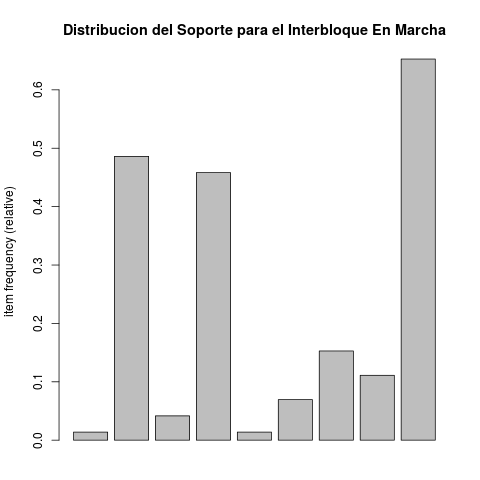
\includegraphics[scale=0.4]{graficos/soportesInterbloquesEnMarcha.png}
\end{center}

En base a la distribución de los datos observada un valor adecuado para el soporte es 0.05.\\

Con esta configuración y luego de eliminar las reglas redundantes se obtuvieron 2 reglas. Se encuentran en el archivo reglasEnMarcha.xml  \\

\begin{center}
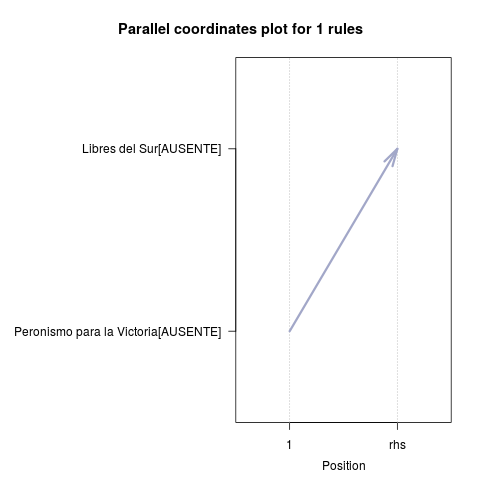
\includegraphics[scale=0.5]{graficos/paracoordEnMarcha.png} \\
\scriptsize{Figura: Debido a la ecala solo puede representarte una de las reglas.} \\
\end{center}

Las reglas obtenidas son \\

{Peronismo para la Victoria[AUSENTE]} $\Longrightarrow${Libres del Sur[AUSENTE]}  \\ 

Con un soporte  de 0.05, confianza 0.8 y lift de 1.64. Esta regla es infrecuente pero muestra que la ausencia del Peronismo Para la victoria tiene una alta correlacion con la ausencia de Libres del Sur. \\ 

{Libres del Sur[POSITIVO]}  $\Longrightarrow${Peronismo para la Victoria[POSITIVO]} \\ 

Con un soporte de 0.40, confianza de 0.87 y lift de 1.34. El voto positivo de Libres del Sur es altamente correlacionado con el voto positivo del Peronismo para la Victoria. \\

\newpage 

\textit{Interbloque contra el resto de los partidos} \\

En base a la distribución de los datos observada un valor adecuado para el soporte es 0.35. \\

Con esta configuración y luego de eliminar las reglas redundantes se obtuvieron 8 reglas. Se encuentran en el archivo reglasEnMarchaRestoPartidos.xml  \\

\begin{center}
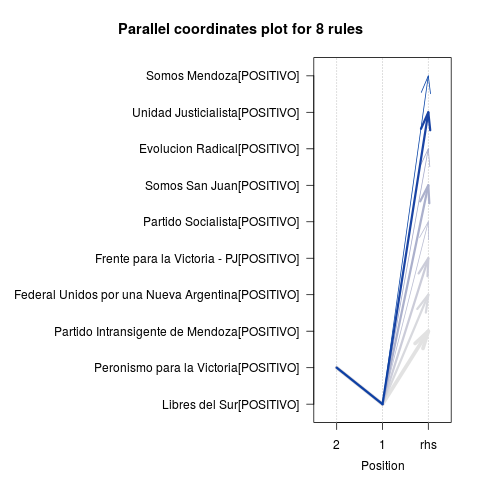
\includegraphics[scale=0.5]{graficos/paracoordEnMarchaPartidos.png} \\
\scriptsize{Figura: La forma en que voto un partido se representa sobre el eje y. Mientras que la intersección sobre  los números representa que se encuentra del lado izquierdo y la flecha representa cual valor se ubica en el lado derecho.} \\
\end{center} 

En este caso todas las reglas obtenidas son consideradas relevantes, ya que muestran los partidos que se alinean con este interbloque con lift supeior a 1 y confianza superior a 0.85. \\

{Libres del Sur[POSITIVO], Peronismo para la Victoria[POSITIVO]} $\Longrightarrow$ {Somos Mendoza[POSITIVO]}  \\

{Libres del Sur[POSITIVO], Peronismo para la Victoria[POSITIVO]} $\Longrightarrow$ {Unidad Justicialista[POSITIVO]} \\

{Libres del Sur[POSITIVO], Peronismo para la Victoria[POSITIVO]} $\Longrightarrow$ {Evolucion Radical[POSITIVO]} \\

{Libres del Sur[POSITIVO], Peronismo para la Victoria[POSITIVO]} $\Longrightarrow$ {Somos San Juan[POSITIVO]} \\

{Libres del Sur[POSITIVO], Peronismo para la Victoria[POSITIVO]} $\Longrightarrow$ {Partido Socialista[POSITIVO]} \\

{Libres del Sur[POSITIVO], Peronismo para la Victoria[POSITIVO]} $\Longrightarrow$ {Frente para la Victoria - PJ[POSITIVO]} \\

{Libres del Sur[POSITIVO], Peronismo para la Victoria[POSITIVO]} $\Longrightarrow$ {Federal Unidos por una Nueva Argentina[POSITIVO]} \\

{Libres del Sur[POSITIVO], Peronismo para la Victoria[POSITIVO]} $\Longrightarrow$ {Partido Intransigente de Mendoza[POSITIVO]} \\

\textbf{Interbloque Argentina Federal}\\

\textit{Dentro del Interbloque} \\

El dataset utilizado es transaccionesargfed.csv. Se analiza la distribución de los datos para encontrar un valor para el soporte del algoritmo apriori. \\

\begin{center}
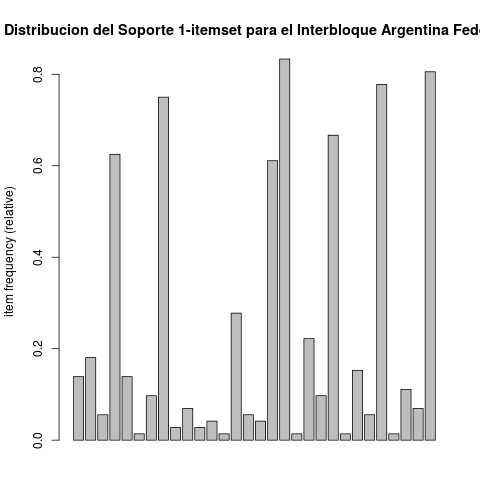
\includegraphics[scale=0.4]{graficos/soportesInterbloquesArgentinaFederal.png}
\end{center}

En base a la distribución de los datos observada un valor adecuado para el soporte es 0.15.\\

Con esta configuración y luego de eliminar las reglas redundantes se obtuvieron 1 reglas, que resulta representativa de todo el bloque. Se encuentra en el archivo reglasInterbloqueArgFed.xml  \\

\begin{center}
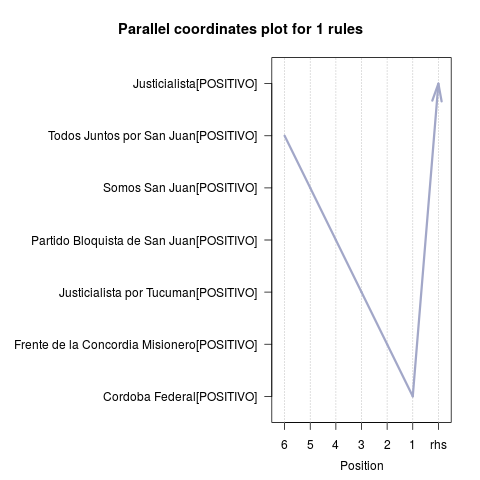
\includegraphics[scale=0.5]{graficos/paracoordArgFed.png} \\
\scriptsize{Figura: La forma en que voto un partido se representa sobre el eje y. Mientras que la intersección sobre  los números representa que se encuentra del lado izquierdo y la flecha representa cual valor se ubica en el lado derecho.} \\
\end{center}   

{Cordoba Federal[POSITIVO], Frente de la Concordia Misionero[POSITIVO], Justicialista por Tucuman[POSITIVO],Partido Bloquista de San Juan[POSITIVO], Somos San Juan[POSITIVO], Todos Juntos por San Juan[POSITIVO]} $\Longrightarrow$ {Justicialista[POSITIVO]} \\

El interbloque vota de forma positiva en conjunto con un lift de 1.2 y confianza 1. \\

\textit{Interbloque contra el resto de los partidos} \\

En base a la distribución de los datos observada un valor adecuado para el soporte es 0.25. \\

Con esta configuración y luego de eliminar las reglas redundantes se obtuvieron 13 reglas. Se encuentran en el archivo reglasArgFedRestoPartidos.xml  \\

\begin{center}
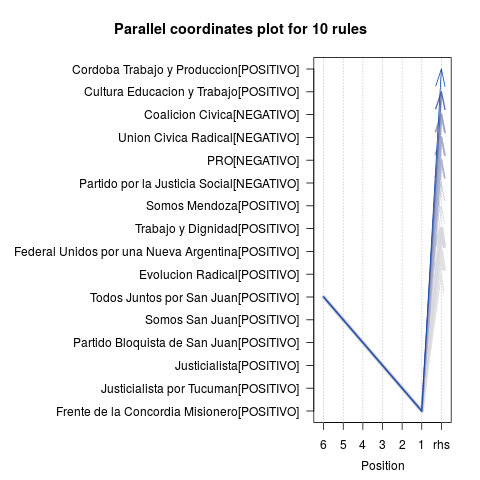
\includegraphics[scale=0.5]{graficos/paracoordArgFedRestoPartidos.png} \\
\scriptsize{Figura: Se presentan las 10 reglas con mayor lift.} \\
\end{center} 

Las reglas que cabe destacar son \\

{Frente de la Concordia Misionero[POSITIVO],Justicialista por Tucuman[POSITIVO], Justicialista[POSITIVO], Partido Bloquista de San Juan[POSITIVO], Somos San Juan[POSITIVO], Todos Juntos por San Juan[POSITIVO]} $\Longrightarrow$ {Frente para la Victoria - PJ[POSITIVO]} \\

Con un soporte de 0.34, confianza de  0.92 y lift 1.12. Si el interbloque completo vota positivo, tambien lo hace el FPV - PJ. \\

{Frente de la Concordia Misionero[POSITIVO],Justicialista por Tucuman[POSITIVO], Justicialista[POSITIVO], Partido Bloquista de San Juan[POSITIVO], Somos San Juan[POSITIVO], Todos Juntos por San Juan[POSITIVO]} $\Longrightarrow$ {PRO[NEGATIVO]} \\

Con un soporte de 0.33, confianza de  0.88 y lift 1.34. Si el interbloque completo vota positivo, el PRO vota negativo. \\

\newpage 

\textbf{Interbloque Frente Renovador - UNA}\\

\textit{Dentro del Interbloque} \\

El dataset utilizado es transaccionesfruna.csv. Se analiza la distribución de los datos para encontrar un valor para el soporte del algoritmo apriori. \\

\begin{center}
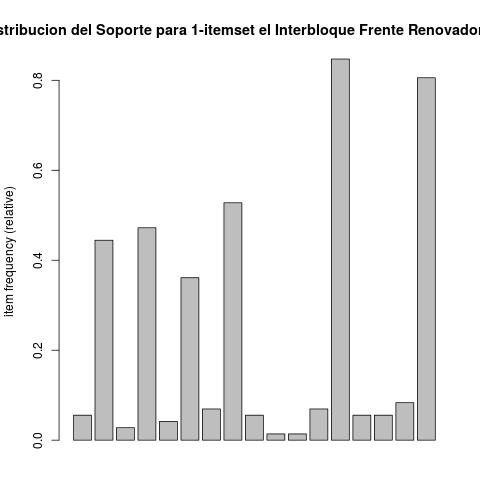
\includegraphics[scale=0.4]{graficos/soportesInterbloquesFrenteRenovador.png}
\end{center}

En base a la distribución de los datos observada un valor adecuado para el soporte es 0.1.\\

Con esta configuración y luego de eliminar las reglas redundantes se obtuvieron 2 reglas, que resulta representativa de todo el bloque. Se encuentra en el archivo reglasFr.xml  \\

\begin{center}
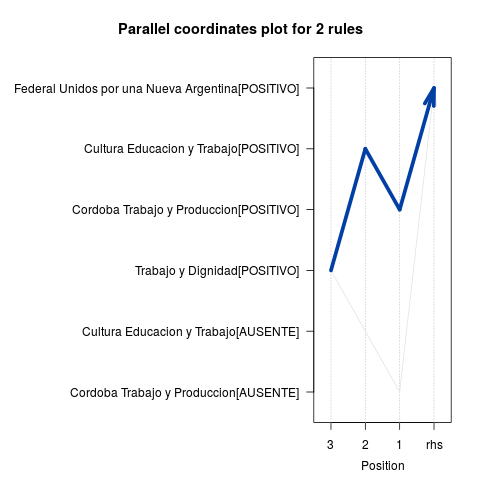
\includegraphics[scale=0.5]{graficos/paracoordFr.png} \\
\scriptsize{Figura: La forma en que voto un partido se representa sobre el eje y. Mientras que la intersección sobre  los números representa que se encuentra del lado izquierdo y la flecha representa cual valor se ubica en el lado derecho.} \\
\end{center} 

La regla que se considera relevante es \\

{Cordoba Trabajo y Produccion[POSITIVO], Cultura Educacion y Trabajo[POSITIVO], Trabajo y Dignidad[POSITIVO]} $\Longrightarrow$ {Federal Unidos por una Nueva Argentina[POSITIVO]} \\

Con un soporte de 0.45, confianza 1 y lift de 1.18. El interbloque vota de forma positiva en conjunto. \\

\textit{Interbloque contra el resto de los partidos} \\

En base a la distribución de los datos observada un valor adecuado para el soporte es 0.25. \\

Con esta configuración y luego de eliminar las reglas redundantes se obtuvieron 18 reglas. Se encuentran en el archivo reglasFrRestoPartidos.xml  \\

\begin{center}
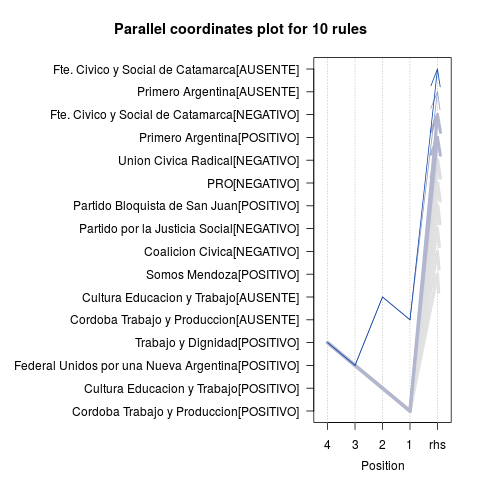
\includegraphics[scale=0.5]{graficos/paracoordFrPartidos.png} \\
\scriptsize{Figura: Se presentan las 10 reglas con mayor lift.} \\
\end{center} 

Las reglas que cabe destacar son \\

{Cordoba Trabajo y Produccio[POSITIVO],Cultura Educacion y Trabajo[POSITIVO],Federal Unidos por una Nueva Argentina[POSITIVO],     Trabajo y Dignidad[POSITIVO]} $\Longrightarrow$ {PRO[NEGATIVO]}  \\

Con un soporte de 0.41, confianza de  0.90 y lift 1.42. Si el interbloque completo vota positivo, el PRO vota negativo. \\

{Cordoba Trabajo y Produccio[POSITIVO],Cultura Educacion y Trabajo[POSITIVO],Federal Unidos por una Nueva Argentina[POSITIVO], Trabajo y Dignidad[POSITIVO]} $\Longrightarrow$ {Frente para la Victoria - PJ[POSITIVO]}  \\

Con un soporte de 0.43, confianza de  0.93 y lift 1.14. Si el interbloque completo vota positivo, tambien lo hace el FPV - PJ . \\


\subsection{Provincias} 

En esta sección se analizan las reglas que involucran a las provincias, el dataset utilizado es $transacciones provincias.csv$ \\

Se calculan las frecuencias para estimar un valor de soporte. \\

\begin{center}
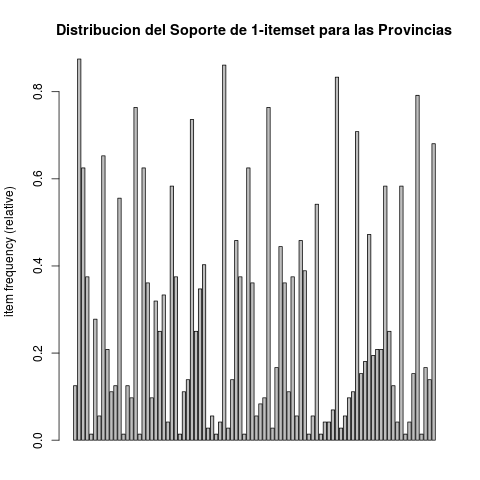
\includegraphics[scale=0.3]{graficos/soportesProvincias.png}
\end{center}

El valor de soporte elegido es de 0.5\\

Se calculan las reglas haciendo prunning sobre las redundantes, obteniendo las maximales y de ahí salen 66 reglas, que se encuentran en el archivo reglasProvincias.xml \\

\begin{center}
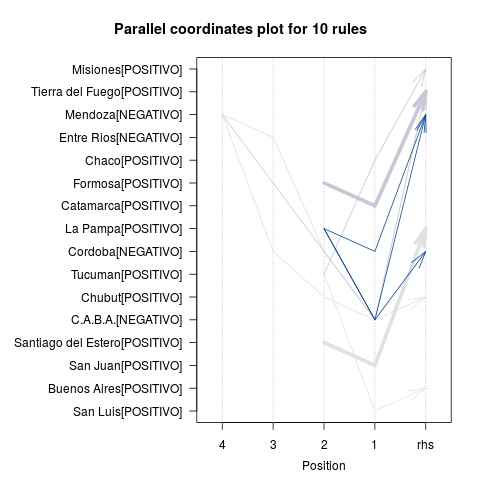
\includegraphics[scale=0.5]{graficos/paracoordProvincias.png} \\
\scriptsize{Figura: Se representan las 10 reglas de mayor lift.}
\end{center} 

En infografialeyes.html pueden visualizarse de forma completa. \\

De las obtenidas cabe destacar: \\

C.A.B.A.[NEGATIVO], Entre Rios[NEGATIVO], Mendoza[NEGATIVO]\\ $\Longrightarrow$ Buenos\ Aires[POSITIVO] \\

{C.A.B.A.[NEGATIVO],                            Cordoba[NEGATIVO],                              Entre Rios[NEGATIVO]}\\ $\Longrightarrow$ {Buenos Aires[POSITIVO]}  \\


Ambas leyes con un soporte de 0.50, confianza 0.87 y lift 1. El voto de la provincia de Buenos Aires es Positivo cuando CABA, Entre Ríos, Mendoza y Córdoba votan en contra de la ley. Esto hace pensar que reduciendo el soporte puede obtenerse una regla con las 4 provincias del lado izquierdo. \\

{C.A.B.A.[NEGATIVO],                            Cordoba[NEGATIVO],                              Entre Rios[NEGATIVO],                           Mendoza[NEGATIVO]}  $\Longrightarrow$ {Chubut[POSITIVO]} \\

Con un soporte de 0.50, confianza 0.90 y lift 1.17.  \\

{C.A.B.A.[NEGATIVO],                            Cordoba[NEGATIVO],                             Entre Rios[NEGATIVO],                           Mendoza[NEGATIVO]} $\Longrightarrow$ {Tierra\ del\ Fuego[POSITIVO]}  \\

Con un soporte de 0.50, confianza 0.90 y lift 1.1.  \\

Las provincias de Chubut y Tierra del Fuego votarán Positivo cuando CABA, Cordoba, Entre Rios y Mendoza voten Negativo. Se puede deducir que sus votos tienden a alinearse en el caso de voto Positivo con Buenos Aires. \\


{Chubut[POSITIVO],                              Formosa[POSITIVO],                              Misiones[POSITIVO],                             Tierra del Fuego[POSITIVO]} $\Longrightarrow$ {San\ Juan[POSITIVO]}  \\    


Con un soporte de 0.50, confianza 0.92 y lift 1.1. \\

{Chubut[POSITIVO],                              Formosa[POSITIVO],                              Misiones[POSITIVO],                             Tierra del Fuego[POSITIVO]} $\Longrightarrow$ {La\ Pampa[POSITIVO]}  \\

Con un soporte de 0.51, confianza 0.94 y lift 1.1. \\

Cuando un voto es positivo en las provincias de Chubut, Formosa, Misiones y Tierra del Fuego, las provincias de San Juan y La Pampa suelen acompañar con su voto positivo. \\


{Formosa[POSITIVO],                             San Juan[POSITIVO],                             Tierra del Fuego[POSITIVO],                     Tucuman[POSITIVO]} $\Longrightarrow$ {Buenos\ Aires[POSITIVO]} \\

Con un soporte de 0.51, confianza 1 y lift 1.14. \\

Cuando el voto es Positivo en las provincias de San Juan, Formosa, Tucuman y Tierra del Fuego, la provincia de Buenos Aires suele acompañar con su voto positivo. \\


\subsection{Partidos y Provincias}

En esta sección se analizan las reglas que involucran a las provincias, el dataset utilizado es $transaccionesprovinciaspartidos.csv$ \\

Se calculan las frecuencias para estimar un valor de soporte. \\

\begin{center}
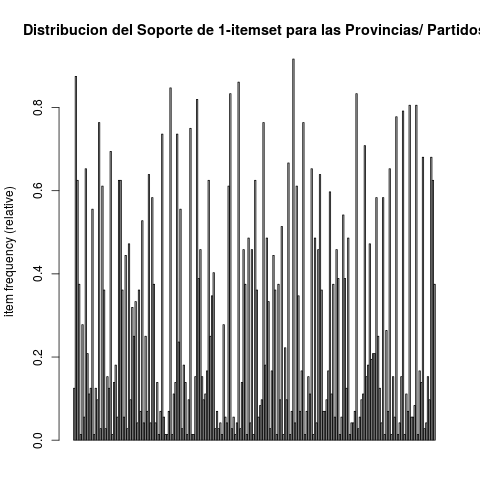
\includegraphics[scale=0.4]{graficos/soportesProvinciasPartidos.png}
\end{center}

El valor de soporte elegido es de 0.60 y en este caso la confianza se elevo al 0.90\\

Se calculan las reglas haciendo prunning sobre las redundantes, obteniendo las maximales y de ahí salen 194 reglas, que se encuentran en el archivo reglasProvinciasPartidos.xml \\


\begin{center}
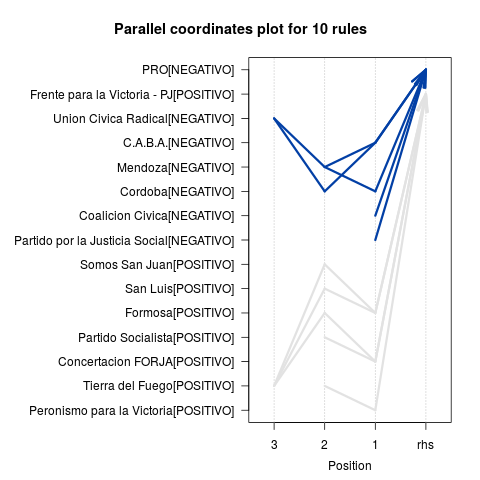
\includegraphics[scale=0.5]{graficos/paracoordProvinciasPartidos.png} \\
\scriptsize{Figura: Se representan las 10 reglas de mayor lift.}
\end{center} 

En infografialeyes.html pueden visualizarse las 100 reglas de mayor lift. \\

{C.A.B.A.[NEGATIVO],        
Mendoza[NEGATIVO], 
Union Civica Radical[NEGATIVO]} $\Longrightarrow$ {PRO[NEGATIVO]} \\

{C.A.B.A.[NEGATIVO],                  Cordoba[NEGATIVO],  Union Civica Radical[NEGATIVO]}  $\Longrightarrow$ {PRO[NEGATIVO]}\\

Ambas reglas con un soporte de 0.61, confianza 1 y lift 1.5. Si la Union Civica Radical y las provincias de CABA, Córdoba y Mendoza votan en negativo, el partido PRO vota en negativo.\\

Esto refuerza reglas antes descriptas donde el voto negativo de la Union Civica Radical estaba altamente correlacionado con el del PRO, que a su vez esta correlacionado con el de CABA. Y el de CABA con las provincias de Mendoza y Córdoba.\\

{Somos San Juan[POSITIVO],                      Todos Juntos por San Juan[POSITIVO],            Trabajo y Dignidad[POSITIVO]}   $\Longrightarrow$ {Buenos Aires[POSITIVO]} \\

Con un soporte de 0.61, confianza 0.97 y lift 1.1. Esta regla tiene la particularidad que el voto de 3 partidos provinciales implica, con una confianza cercana a 1, el voto de la provincia con más diputados. \\

{La Pampa[POSITIVO],                            San Luis[POSITIVO],                             Tierra del Fuego[POSITIVO]}  $\Longrightarrow$ {Partido Intransigente de Mendoza[POSITIVO]} \\

Con un soporte de 0.61, confianza 1 y lift 1.09. El voto de un partido provincial de Mendoza puede estimarse al voto de 3 provincias distintas a las del partido.\\


{San Juan[POSITIVO],                            Somos San Juan[POSITIVO],                       Todos Juntos por San Juan[POSITIVO]}    $\Longrightarrow$ {Justicialista[POSITIVO]}  \\

Con un soporte de 0.61, confianza 0.95 y lift 1.14. Los votos de dos partidos provinciales de San Juan junto con la provincia, alcanzan para estimar el voto del partido Justicialista que tiene alcance nacional. \\

\subsection{Sanciones de Ley}

Para concluir el análisis de las reglas detrás de las votaciones en el Congreso, se analizan las votaciones que lleva a que una ley sea aprobada. Para esto se utiliza el dataset del archivo $transacciones.csv$ para generar reglas que el lado derecho sea $LEYAPROBADA$ o $LEYRECHAZADA$ y sean de la longitud máxima que fue posible computar. \\

El objetivo fue verificar que se mantengan las reglas obtenidas a partir de los subdataset.  \\

La longitud máxima que se pudo computar fueron reglas de longitud 17, es decir 16 items del lado izquierdo y 1 del lado derecho. Se tomo como soporte 0.4 y confianza de 0.90.  \\

Se obtuvieron 2 reglas que se encuentran en el archivo reglasLeyes.xml. Y pueden visualizarse de forma completa las relaciones en infografialeyes.html.\\

Las reglas obtenidas son \\

\begin{center}
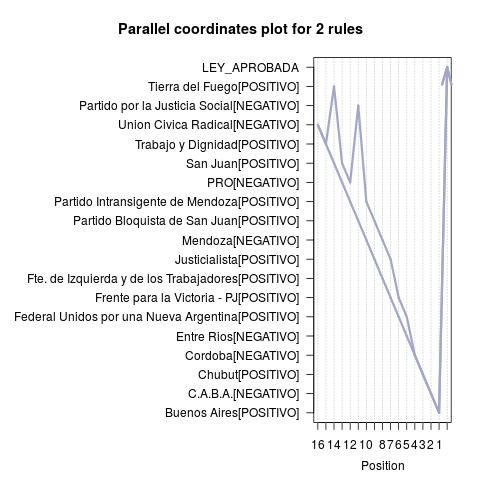
\includegraphics[scale=0.5]{graficos/paracoordLeyes.png} \\
\end{center} 

Para la interpretación de estas leyes se repasaron los casos de estudio anteriores, complementando con el material de la infografía. \\

{Buenos Aires[POSITIVO],                    
C.A.B.A.[NEGATIVO],                         
Chubut[POSITIVO],                           
Cordoba[NEGATIVO],                          
Entre Rios[NEGATIVO],                       
Federal Unidos por una Nueva Argentina[POSITIVO],                       
Frente para la Victoria - PJ[POSITIVO],     
Fte. de Izquierda y de los Trabajadores[POSITIVO],  
Justicialista[POSITIVO],                    
Mendoza[NEGATIVO],  
Partido Bloquista de San Juan[POSITIVO],    
Partido Intransigente de Mendoza[POSITIVO], 
PRO[NEGATIVO], 
San Juan[POSITIVO],
Trabajo y Dignidad[POSITIVO],            
Union Civica Radical[NEGATIVO]}                 $\Longrightarrow$ {LEY APROBADA} \\

Con un soporte de 0.40, confianza de 0.96 y lift de 1.14. De los previos análisis se puede observar que se mantiene coordinada la votación Negativa de las provincias de CABA, Cordoba, Entre Ríos y Mendoza, además de la de PRO y la Union Civica Radical. Vuelve a repetirse la oposión de la provincia de Buenos Aires con CABA y del PRO con el Frente para la Victoria - PJ. También se mantiene la relación de voto positivo entre Fte. de Izquierda y de los Trabajadores y Frente para la Victoria - PJ, además de la relación del Frente para la Victoria - PJ con los otros partidos mayoritarios, Federal Unidos por una Nueva Argentina y Justicialista. Los partidos provinciales de San Juan y la provincia votan de forma igual que la provincia de Buenos Aires. \\

{Buenos Aires[POSITIVO],
C.A.B.A.[NEGATIVO], 
Chubut[POSITIVO], 
Cordoba[NEGATIVO], 
Federal Unidos por una Nueva Argentina[POSITIVO],
Frente para la Victoria - PJ[POSITIVO], 
Justicialista[POSITIVO],
Mendoza[NEGATIVO], 
Partido Bloquista de San Juan[POSITIVO],
Partido Intransigente de Mendoza[POSITIVO],
Partido por la Justicia Social[NEGATIVO],
PRO[NEGATIVO],              
San Juan[POSITIVO],  
Tierra del Fuego[POSITIVO], 
Trabajo y Dignidad[POSITIVO],  
Union Civica Radical[NEGATIVO]}     $\Longrightarrow$ {LEY APROBADA} \\

Con un soporte de 0.40, confianza de 0.96 y lift de 1.14. A las relaciones vistas en la ley anterior cabe también agregar que se mantiene el voto positivo de Tierra del Fuego cuando CABA, Cordoba, Entre Ríos y Mendoza votan de forma negativa. \\

\newpage 

\section{Conclusiones}
Fue posible establecer ciertas reglas que acompañan la dinámica de la votaciones en la Cámara Baja.
En esta sección, se presentan las conclusiones obtenidas.

\begin{description}
\item[$\bullet$] Es muy importante entender qué reglas se quieren obtener para poder pensar como armar las transacciones. En este caso, existen muchas reglas posibles que se pueden obtener y cada una da cierta información, pero para poder llegar a ellas, se necesitan transacciones que lo permitan (corriendo el álgoritmo \textit{apriori}).
\item[$\bullet$] Otra cosa importante, es entender el negocio al que pertenecen los datos a analizar. En este caso, son votos de diputados, que pertenecen a bloques y representan a provincias. Es decir, para realizar este trabajo es necesario entender la coyuntura politica argentina. De lo contrario, es muy dificil entender cuando una regla es redundante, cuando una regla es \textit{sorpresiva}, cuando una regla era esperada. Otra cosa que nos vimos, fue que algunos partidos se cambiaban el nombre o se aliaban con otros, y a la hora de analizar el dataset y crear las transacciones es importante tenerlo en cuenta.
\item [$\bullet$] Además de entender el negocio, se necesita entender qué es lo que se está observando en el dataset. La mayoria de las reglas generadas tiene confianza 1, y eso ocurre por como son las votaciones en argentina. Es por eso, que para decidir el \textit{minsup} tuvimos que generar un gráfico que nos explique la distribución de los soportes. \\
\end{description} 

Por otro lado, tenemos las conclusiones que obtenemos de las reglas más destacadas que obtuvimos:

\begin{description}

\item[$\bullet$] Los diputados votan en sintonía con los demás miembros de su partido. Sin importar la provincia a la que pertenezcan.

% Interbloque PRO sintonia
\item[$\bullet$] Cuando se analiza reglas de longitud 2, el interbloque Cambiemos se muestra en sintonía. Cuando se analiza con reglas de mayor longitud, se ve que a la hora de votar \textit{positivo} tambien hay sintonia aunque algunas veces el Frente Civico Social de Catamarca y Salta Somos Todos se ausentan. A la hora de votar \textit{negativo}, Salta Somos Todos suele salir de esa sintonía y votar positivo. A pesar de esto, el Movimiento Popular Neuquino suele acompañar al interbloque con su voto negativo.

% PRO vs FPV
\item[$\bullet$] Por lo general, cuando el PRO vota negativo, el FPV vota positivo, confirmando lo que uno ve en la politica. Esto se extiende cuando vemos que el interbloque cambiemos vota negativo (excepto Salta Somos Todos, como menionamos anteriormente), el FPV - PJ vota positivo.

% Sintonia Peronismo
\item[$\bullet$] Hay una gran sintonía en los partidos englobados por el \textit{peronismo}.

% 3 interbloques distintos
\item[$\bullet$] Sorpresivamente, hay una sintonía entre el Partido Socialista, Somos San Juan y Federal Unidos por una Nueva Argentina. Lo llamativo es que los 3 partidos pertenecen a interbloques distintos.

% Partido Intr Mendoza con oposicion
\item[$\bullet$] El Partido Intrsansigente de Mendoza, que no pertenece a ningún interbloque, suele votar positivo cuando los partidos mayoritarios de la oposición votan positivo. Esto indica que la división de interbloques no muestra la totalidad de \textit{alianzas}.

% Partidos mayoritarios juntos
\item[$\bullet$] Por lo general, si el FPV - PJ vota positivo, entonces el partido Justicialista y el partido Federal Unidos por una Nueva Argentina tambien lo hagan. Lo sorprendnte de esto es que son 3 de los 4 partidos más grandes (a nivel cantidad de diputados) y cuando estos 3 votan lo mismo, pueden determinar el resultado de la ley en cuestión.

\end{description}

\section{Referencias Bibliográficas}

\begin{description}
\item[$\bullet$]Material de la materia: Reglas de Asociación y Patrones Secuenciales - Profesora: Cecilia Ana Ruz - Universidad de Ciencias Exactas y Naturales.
\end{description}

\end{document}
